\documentclass{birkjour}

\usepackage{amsmath}
\usepackage{amssymb}
\usepackage{amsthm}
\usepackage{graphicx}
\usepackage{float}
\usepackage{url}

\newtheorem{thm}{Theorem}[section]
 \newtheorem{cor}[thm]{Corollary}
 \newtheorem{lem}[thm]{Lemma}
 \newtheorem{prop}[thm]{Proposition}
 \theoremstyle{definition}
 \newtheorem{defn}[thm]{Definition}
 \theoremstyle{remark}
 \newtheorem{rem}[thm]{Remark}
 \newtheorem*{ex}{Example}
 \numberwithin{equation}{section}

\newcommand{\G}{\mathbb{G}}
\newcommand{\V}{\mathbb{V}}
\newcommand{\Vb}{\mathbb{\overline{V}}}
\newcommand{\W}{\mathbb{W}}
\newcommand{\R}{\mathbb{R}}
\newcommand{\Alpha}{A}

\begin{document}

\title{A Model For Quadric Surfaces\\Using\\Geometric Algebra}

\author{Spencer T. Parkin}
\email{spencer.parkin@gmail.com}

\numberwithin{equation}{section}

\subjclass{Primary 14J70; Secondary 14J29}

\keywords{Quadric Surface, Geometric Algebra, Quadric Model}

% add ref for tranforming quadric surface and intersecting quadric surfaces.
% use "http://science.kennesaw.edu/~plaval/math2203/func3d.pdf" to talk
% about how we might classify quadrics differently in this model.

%\dedicatory{To Melinda and Naomi}

\begin{abstract}
Inspired by the conformal model of geometric algebra,
a similar model of geometry is developed for the set
of all quadric surfaces in $n$-dimensional space.  Bivectors of the geometric algebra
are found to be representative of quadric surfaces.  Coordinate free canonical forms
of such bivectors are found for common quadric surfaces.  The model is investigated
for usefulness and compared to the conformal model.
\end{abstract}

\maketitle

\section{The Construction Of The Model}\label{sec_ga_construct}

The stage for this model of $n$-dimensional quadric surfaces is set in the geometric
algebra we'll denote by $\G$ that is generated by a Euclidean vector space $\W$ of dimension
$2(n+1)$.  Letting $\{e_i\}_{i=0}^{2n+1}$ be an orthonormal set of basis vectors
generating $\W$, we let $\{e_i\}_{i=0}^n$ be such a set of vectors generating
the $(n+1)$-dimensional vector sub-space $\V$ of $\W$ upon which we'll impose the
usual interpretation of $(n+1)$-dimensional homogeneous space.  Specifically,
a vector $v\in\V$ with $v\cdot e_0\neq 0$ represents the point given by\footnote{Throughout this
paper we let the outer product take precedence over the inner product, and the geometric product
take precedence over both the inner and outer products.}
\begin{equation}
\frac{e_0\cdot e_0\wedge v}{e_0\cdot v}
\end{equation}
in $n$-dimensional Euclidean space, imposing the usual correlation between $n$-dimensional
vectors and $n$-dimensional points.\footnote{The correlation between
vectors and points spoken of here is that of having a vector represent the point
at its tip when its tail is placed at the origin.}  We will take the liberty of letting vectors $v\in\V$ with $v\cdot e_0=0$
represent points under the same interpretation of which has just been spoken, as
well as pure directions with magnitude.  The intended interpretation will be made clear
in the context of our usage.  We will refer to all vectors $v\in\V$ with $v\cdot e_0\neq 0$
as affine points, and such vectors with $v\cdot e_0=0$ as Euclidean points
or sometimes directions.  See section 2.1.1 of \cite{Birchfield98} for a great introduction to
homogeneous coordinates.

We now introduce a function defined on $\G$ having the outermorphic property.
This means that it is a linear function and that it preserves the outer product.  We will
use over-bar notation to denote the use of this function.  Doing so, for any
element $E\in\G$, we define $\overline{E}$ as
\begin{equation}
\overline{E} = SE\tilde{S},
\end{equation}
where the rotor $S$ is given by
\begin{equation}
S = 2^{-(n+1)/2}\prod_{i=0}^n\left(1-e_ie_{i+n+1}\right),
\end{equation}
and $\tilde{S}$ denotes the reverse of $S$.
As the reader can check, for any integer $i\in[0,n]$, we have $\overline{e_i}=e_{i+n+1}$,
and similarly, $\overline{e_{i+n+1}}=-e_i$.
The rotor $S$ simply rotates any element taken from the geometric algebra generated
by $\V$, (which we'll denote by $\G(\V)$), into the identical geometric
algebra generated by the vector
space we'll denote by $\overline{\V}$ that is complement to $\V$ with respect to $\W$.
The over-bar function is an isomorphism between the geometric algebras $\G(\V)$ and $\G(\overline{\V})$.
We will find the over-bar function convenient when performing algebraic manipulations in our model
to the extent that in many cases we can forget about the versor $S$, letting the over-bar notation be nothing
more than a device used to distinguish between elements of $\G(\V)$ and $\G(\overline{\V})$.

The geometric algebra $\G$ that we have constructed here is similar to ``the mother algebra''
in \cite{DoranHestenes93}, except that while $\G(\V)$
is Euclidean, so is the geometric algebra $\G(\overline{\V})$.  We do not
make use of an anti-Euclidean geometric algebra.  Although doing so might prove beneficial,
it is worth forgoing for now in the realization that $\G$, as it stands, and as we'll see, sufficiently
fulfills at least the minimum requirements of a model for quadric surfaces.

We are now ready to give the definition by which we will interpret bivectors in $\G$
as $n$-dimensional quadric surfaces.  It is as follows.
For any element $E\in\G$, we say that $E$ is representative of the $n$-dimensional
quadric surface generated by the set of all affine points $p\in\V$ such that
\begin{equation}\label{equ_quadric_condition}
0 = p\wedge\overline{p}\cdot E.
\end{equation}

Notice that when $\mbox{grade}(E)>1$, there is no ambiguity, despite the non-associativity
of the inner product, in rewriting equation
\eqref{equ_quadric_condition} as
\begin{equation}
0 = p\cdot E\cdot\overline{p},
\end{equation}
which resembles a sort of conjugation of $E$ by $p$.  This may perhaps be a more
familiar form for readers familiar with the study of quadric surfaces in projective geometry.
For example, see equation (1) of the chapter on quadric surfaces in \cite{MehlhornYap04}.
Also notice that we have not required that $E$ be a bivector in definition \eqref{equ_quadric_condition},
because we may find this condition useful and meaningful for any element of $\G$.  For now,
however, we will restrict our attention to the case when $E$ is a bivector.

To see why definition \eqref{equ_quadric_condition} works, simply notice that when $E$ is a bivector, we have
\begin{equation}\label{equ_homogeneous_polynomial}
p\wedge\overline{p}\cdot E=\sum_{i=0}^n\sum_{j=i}^n \lambda_{ij}(p\cdot e_i)(p\cdot e_j),
\end{equation}
which we can recognize as a homogeneous polynomial of degree 2 in the vector components of $p$.
The scalars $\lambda_{ij}$, with $0\leq i\leq j\leq n$, may be formulated in terms of $E$ by
\begin{equation}\label{equ_quadric_components}
\lambda_{ij} = \left\{\begin{array}{ll}
e_i\overline{e_j}\cdot E & \mbox{if $i=j$,} \\
\left(e_i\overline{e_j}+e_j\overline{e_i}\right)\cdot E & \mbox{if $i\neq j$.}
\end{array}\right.
\end{equation}
It should be noted that bivectors do not uniquely represent quadric surfaces, not even up to scale.
This is apparent from equation \eqref{equ_quadric_components} when we see that for $i\neq j$,
we can freely choose certain components of the bivector without changing the represented
quadric so long as their sum is still $\lambda_{ij}$.  The problem this may pose in our model
comes from a very important result in the conformal model.  In the conformal model, if
two blades are known to represent the same non-trivial geometry in the same way,
then it can be shown that the two blades are equal, up to scale.
In our present model, it may take more than just
multiplying by a non-zero scalar factor to get a bivector known to represent a certain geometry in a
known canonical form.  To account for this during the performance of algebraic manipulations,
we will introduce the following notation.  We will say that quadrics $E_a$ and $E_b$ are
equivalent, writing $E_a\equiv E_b$, whenever $E_a$ and $E_b$ represent the same quadric
under definition \eqref{equ_quadric_condition}.  For example, for any two vectors $u,v\in\V$, we have
\begin{equation}
u\wedge\overline{v}\equiv -2u\wedge\overline{v}\equiv u\wedge\overline{v}+v\wedge\overline{u}
\equiv(u+\overline{v})\wedge(u-\overline{v}).
\end{equation}
Be aware that if $E=E_a+E_b$ and $E_a\equiv E_c$, then this does not imply that $E\equiv E_b+E_c$
unless it can be shown that for all affine points $p\in\V$, we have
\begin{equation}
p\wedge\overline{p}\cdot E_a=p\wedge\overline{p}\cdot E_c.
\end{equation}
This condition is weaker than $E_a=E_c$ yet stronger than $E_a\equiv E_c$.

Another important difference to point out here between our present model and the conformal model is that,
unlike what we can analogously expect from the point-definition of the conformal model,
here the 2-blade form $a\wedge\overline{a}$ found in definition \eqref{equ_quadric_condition}, for
any affine point $a\in\V$ not at origin, does not represent the affine point $a$ under definition \eqref{equ_quadric_condition}.
In homogenized form, the affine point represented by $a\wedge\overline{a}$ is given by
\begin{equation}
e_0 - \left(\frac{e_0\cdot e_0\wedge a}{e_0\cdot a}\right)^{-1},
\end{equation}
which is the reflection about the origin of the spherical inversion of the affine point $a$
about the unit-sphere centered at the origin.  The affine point $e_0$ at the origin
simply represents the empty point-set geometry, or the geometry of nothing.  It is also
easy to see that $a\wedge\overline{a}$ does not represent the affine point $a$, because there are no
null blades in our purely Euclidean geometric algebra $\G$.

\section{The Construction Of Quadric Surfaces In The Model}

Having constructed our model, we are now ready to find canonical forms of bivectors
representing a variety of well-known quadric surfaces.  Our approach here will be
similar to that taken in Section 3 of \cite{Miller87}.

Let us begin with the
spheroid, (a special case of ellipsoid), the circular cylinder, and the circular hyperboloid
of one sheet.  We will find that all of these surfaces share the same canonical form,
because they may all be characterized as the Euclidean point solution set of the equation
\begin{equation}\label{equ_spheroid}
0 = -r^2 + (x-c)^2 + \lambda((x-c)\cdot v)^2
\end{equation}
in the Euclidean point $x\in\V$, where $c\in\V$ is a Euclidean
point denoting the center of the surface, $v\in\V$ is a unit-length direction
vector, $r\in\R$ is the radius of the geometry about the axis $v$ at $c$, and
$\lambda\in\R$ is a scalar indicating the type and extremity of the surface.
Specifically, if $\lambda<-1$, we get a circular hyperboloid of one sheet;
if $\lambda=-1$, we get a circular cylinder; if $-1<\lambda<0$, we get a stretched
sphere; if $\lambda=0$, a sphere; and if $\lambda>0$, a squished sphere.  Interestingly,
when $r=0$ and $\lambda<-1$, we get circular conical surfaces; a right-circular conical
surface if $\lambda=-2$.

Expanding equation \eqref{equ_spheroid}, we get
\begin{equation}
0 = x^2 + \lambda(x\cdot v)^2 - 2x\cdot (c+\lambda(c\cdot v)v) + c^2 + \lambda(c\cdot v)^2 - r^2,
\end{equation}
from which it is possible to factor out $-p\wedge\overline{p}$
in terms of the inner product, where $p=e_0+x$
is a homogenized affine point.  Doing so, we see that the bivector
$E$ given by
\begin{equation}\label{equ_spheroid_bivector}
E = \Omega + \lambda v\wedge\overline{v} - 2(c+\lambda(c\cdot v)v)\wedge\overline{e_0} + (c^2+\lambda(c\cdot v)^2-r^2)A,
\end{equation}
is representative of the three surface types by definition \eqref{equ_quadric_condition}, where the constant
$\Omega$ is defined as
\begin{equation}
\Omega=\sum_{i=1}^n e_i\overline{e_i},
\end{equation}
and $A$ is the constant defined as $A=e_0\overline{e_0}$.  We will find each of these useful as
frequently recurring constants in our calculations.

Such forms as that in equation \eqref{equ_spheroid_bivector} are useful, not only
for composition, but especially decomposition in the cases
where we have formulated what may, for example, be a spheroid by some means
other than composition.
This gives the model power as an analytical tool.  If we can solve a problem whose solution
is a bivector known to represent a spheroid, then we can use this canonical form to answer
questions about that spheroid.  Where is its center?  What is its axis?  What is its radius
about that axis?  As is often the case in mathematics, however, decomposition is
harder than composition.  A general sequence of decomposition steps for the
form \eqref{equ_spheroid_bivector} is not obvious, if it exists, but we will
proceed now to give such a sequence for the case when $E$ is known
to be a cylinder.  That is, when $\lambda=-1$.

The first thing to notice is that the canonical form $E$ in equation \eqref{equ_spheroid_bivector}
is in a homogenized form, because the coeficient of $\Omega$ is 1.  Looking at any canonical form,
if there exists a term in that form with a consistent magnitude, (a magnitude that does not change
with any instantiation of that form with a given set of parameters), then we can usually find a way
to homogenize that form -- the process by which we transform any non-homogenized element $E'$
known to represent the same quadric as that of a homogenized and canonical form $E$ into $E$.
For the canonical form \eqref{equ_spheroid_bivector} with $\lambda=-1$, a common\footnote{Recall
that it may take more than multiplying by a simple scalar factor to homogenize a bivector in $\G$
as discussed in Section~\ref{sec_ga_construct}.}
non-homogenized form is given by
\begin{equation}
E' = \omega(\Omega - v\wedge\overline{v}-2u\wedge\overline{e_0}+(u^2-r^2)A),
\end{equation}
where $u=c-(c\cdot v)v$, $\omega\neq 1$ and $\omega\neq 0$.  To find the homogenized form $E=E'/\omega$,
it is not hard to show that
\begin{equation}
\omega = -\frac{\Omega\cdot E'}{n-1}.
\end{equation}
We can then proceed to decompose the canonical form $E$ as follows.

We start by recovering the unit-length direction vector $v$.  This can be
done as
\begin{equation}
v = \sum_{i=1}^n\left(e_i-\overline{e_i\wedge e_0\cdot e_0\wedge E}\right).
\end{equation}
It is unfortunate that we had to refer to a basis to obtain $v$; nevertheless,
it is done.  The rest of the decomposition will proceed with greater satisfaction.

There is no way to recover $c$ for cylinders, which is quite obvious.
The choice for the point $c$, the center of the cylinder, may be arbitrarily
chosen as any point along its spine.  This information is lost in composition,
so we may therefore arbitrarily choose
\begin{equation}
c=-\frac{1}{2}A\cdot(E\wedge e_0)
\end{equation}
as the cylinder's center, which, incidentally, will also be the point on the spine of
the cylinder closest to the origin.

Lastly, we may find the radius of the cylinder from the simple equation
\begin{equation}
r^2 = c^2 + A\cdot E.
\end{equation}

A generalization of equation \eqref{equ_spheroid} should be mentioned
before moving on.  It is given by
\begin{equation}
0 = -r^2 + (x-c)^2 + \sum_{i=1}^k \lambda_i((x-c)\cdot v_i)^2,
\end{equation}
which would probably give us the general set of ellipsoids, provided
the set of $k$ direction vectors in $\{v_i\}_{i=1}^k$ are
linearly independent.

The following table summarizes a few additional canonical forms.
\begin{equation}\label{equ_canonical_forms_table}
\begin{array}{|l|l|}
\hline
\mbox{Geometry} & \mbox{Canonical/Homogenized Form} \\
\hline
\mbox{Plane} & v\wedge\overline{e_0} - (c\cdot v)A,\;|v|=1 \\
\hline
\mbox{Sphere} & \Omega - 2c\wedge\overline{e_0} + (c^2-r^2)A \\
\hline
\mbox{Point} & \Omega - 2c\wedge\overline{e_0} + c^2A \\
\hline
\mbox{Line} & \Omega - v\wedge\overline{v} - 2u\wedge\overline{e_0} + u^2A,\;u=c-(c\cdot v)v \\
\hline
\mbox{Plane-Pair} & ((c_a\cdot v_a)e_0-v_a)\wedge((c_b\cdot v_b)\overline{e_0}-\overline{v_b}) \\
\hline
\end{array}
\end{equation}
For the plain-pair form in table \eqref{equ_canonical_forms_table}, $c_a,c_b\in\V$ are Euclidean points
on the two planes, and $v_a,v_b\in\V$ are direction vectors normal to each of the two planes.

% What about circles and point-pairs of the conformal model?  Are they found in our model?

\section{Making Use Of The Model}

Admittedly, there is really nothing interesting about this model unless we can
prove that it has some utility.  The conformal model, for example, has at least
two great features.  The first is the utility of the wedge product in generating
intersections between geometries in dual form, or point-fitting between
geometries in direct form.  It is even possible to
make use of dual imaginary intersections by reinterpreting them as real geometries
in direct form.  The second great feature of the conformal model is the
surprising fact that all geometries in the conformal model are, as versors, also conformal transformations
with geometric significance relative to the simultaneously represented geometry.
Then, realizing that all conformal geometries, (with the exception of flat points), have
a factorization in direct form as an outer product of points, the outermorphic
property of versor conjugation allows us to predict the action of any versor
transformation on almost any conformal geometry.

These are great features!  But what can the model at present do for us?  Well,
the first observation we must make is that the set of all known quadrics
is represented by the set of all bivectors in $\G$, under-which the inner
and outer products are obviously not closed.  Only addition and subtraction
are closed in this set, and so we're left to wonder what we might be able
to prove about the addition and subtraction of $n$-dimensional quadric surfaces.
Letting $B_a,B_b\in\G$ be bivectors, it is not hard to see that $B_a\pm B_b$, under
definition \eqref{equ_quadric_condition}, must represent at least the intersection, if any,
of the quadric surfaces $B_a$ and $B_b$, but this is not an exact answer to the
question of what surface $B_a\pm B_b$ represents.

Let's try an example.  Suppose $B_a$ and $B_b$ are both homogenized spheres with
a real intersection and having
Euclidean centers $c_a,c_b\in\V$, respectively.  Let $r_a,r_b\in\R$
be the respective radii of $B_a$ and $B_b$.  It then follows from
table \eqref{equ_canonical_forms_table} that $B_a-B_b$, in homogenized
form, is given by
\begin{equation}\label{equ_diff_of_spheres}
\frac{v}{|v|}\wedge\overline{e_0}-\left(\frac{v}{|v|}\cdot\frac{c_a+c_b+(r_b^2-r_a^2)v^{-1}}{2}\right)A,
\end{equation}
where $v$ is the vector $c_a-c_b$, which, again by table \eqref{equ_canonical_forms_table},
tells us that this is a plane with normal $v$.  A point on the plane is also apparent from
\eqref{equ_diff_of_spheres}, namely $(c_a+c_b+(r_b^2-r_a^2)v^{-1})/2$.
Then, knowing that $B_a-B_b$ must contain the intersection of the
two spheres, we can conclude that this point must be in the plane containing the circle that is
the intersection of the two spheres, because $B_a-B_b$ must be the said plane.  Notice
that even if the spheres don't intersect, we still get a meaningful result.  A picture of
$B_a-B_b$ is given in Figure~\ref{fig_diff_of_spheres}.

\begin{figure}
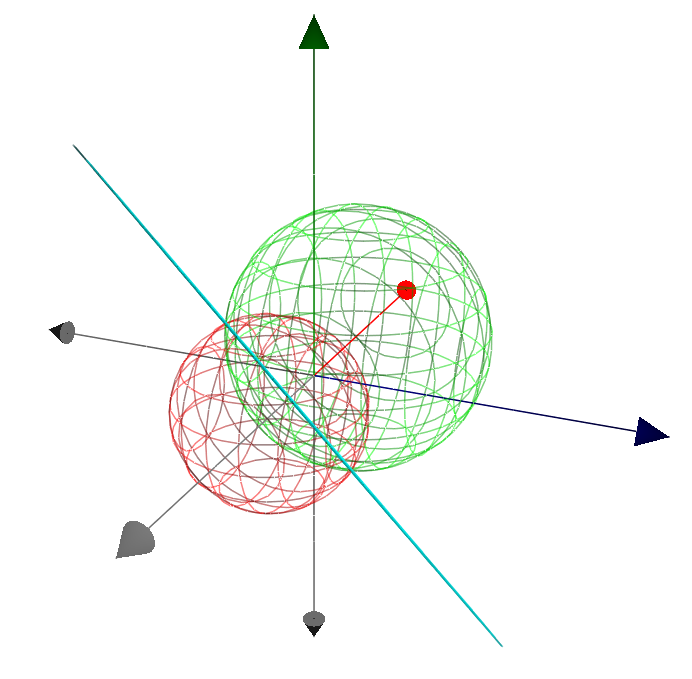
\includegraphics[scale=0.5]{DiffOfSpheres}
\caption{The difference of two homogenized spheres gives the plane, shown here on edge,
containing their intersection.  The spheres were rendered as a number of traces in
various parallel planes.}
\label{fig_diff_of_spheres}
\end{figure}

At first sight, the sum of a sphere and a plane may not seem that interesting.
However, the sum of a homogenized sphere and a non-homogenized plane is
interesting, because the result is always a sphere in homogenized form.  The
scalar amount at which the plane is non-homogenized simply indicates twice
the length along the normal of the plane that the center of the original sphere
is displaced in the opposite direction of that normal to find a sphere intersecting the
plane in the same circle as that of the original sphere.

Interestingly, the difference of spheres generalizes to the idea of subtracting
spheroids.  A picture of this is given in Figure~\ref{fig_diff_of_spheroids}.
Of course, there is undoubtedly a geometric significance in the difference
between any two homogenized quadric surfaces containing $\Omega$.  It
would be interesting to find out exactly what that is.  The sum of such
elements is also interesting.  For example, in the case of two homogenized
points, it can be shown that their sum is the imaginary sphere having the
two points as opposite poles.  Specifically, we have
\begin{align}
 & \left(\Omega-2a\wedge\overline{e_0}+a^2\Alpha\right) +
\left(\Omega-2b\wedge\overline{e_0}+b^2\Alpha\right) \\
\equiv\;& \Omega-2\left(\frac{a+b}{2}\right)\wedge\overline{e_0} +
\left(\left(\frac{a+b}{2}\right)^2+\left(\frac{a-b}{2}\right)^2\right)\Alpha,
\end{align}
where $a,b\in\V$ are Euclidean points, which we can recognize
from table \eqref{equ_canonical_forms_table} as an imginary sphere.

\begin{figure}
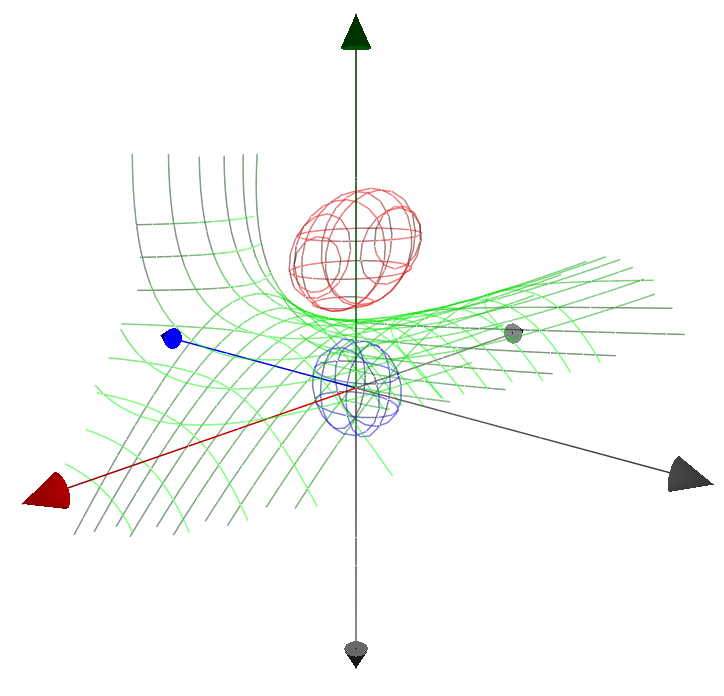
\includegraphics[scale=0.5]{DiffOfSpheroids}
\caption{The difference of two homogenized spheroids gives a hyperbolic paraboloid.
In this case, the two paraboloids have no real intersection.}
\label{fig_diff_of_spheroids}
\end{figure}

\section{Intersecting Quadric Surfaces}

% LEVIN, J. A parametric algorithm for drawing pictures of solid objects composed of quadric
% surfaces. Commun. ACM 19,lO (Oct. 1976).

% SARRAGA, R. F. Algebraic methods for intersections of quadric surfaces in GMSOLID. Comput.
% Vision Graph. Image Process. 22, 2 (May 1983).

In this section we briefly consider the ability to intersect quadric surfaces in the model.
A desire to do such a thing is motivated by an ability to do it in the conformal model,
and by its applications to drawing solid objects composed of quadric surfaces.  (See \cite{Levin76}, \cite{WangGoldmanTu03}
and \cite{Miller87}.)  After finding vectors dually representative of planes and spheres,
the ability to intersect such geometries is one method of the conformal model for generating
all geometries of that model.  We have seen how the model at present is capable of representing
planes and spheres, so naturally we would wish to intersect them.

Noticing that any trivector $T\in\G$ can be written in the form
\begin{equation}
T = \sum_{i=1}^k v_i\wedge B_i,
\end{equation}
where $\{v_i\}_{i=1}^k\subset\W$ is a set of $k$ vectors and $\{B_i\}_{i=1}^k\subset\G$
is a set of $k$ bivectors, we may proceed to apply definition \eqref{equ_quadric_condition}
to find that
\begin{equation}\label{equ_trivector_geo}
0 = p\wedge\overline{p}\cdot T =
p\cdot\sum_{i=1}^k(\overline{p}\cdot v_i)B_i -
\overline{p}\cdot\sum_{i=1}^k(p\cdot v_i)B_i +
\sum_{i=1}^k(p\wedge\overline{p}\cdot B_i)v_i,
\end{equation}
showing that $T$ is representative of the quadric surface that is the intersection
of all quadrics in $\{B_i\}_{i=1}^k$, provided that $\{v_i\}_{i=1}^k$ is a linearly
independent set of vectors, and that for all affine points $p\in\V$, and for any
integer $i\in[1,k]$, we have $p\cdot v_i=\overline{p}\cdot v_i=0$.  This last condition,
unfortunately, cannot be satisfied in $\G$ as we have defined it, nor does it seem
practical or reasonable to extend $\G$ in a way that makes the condition possible,
mainly because the resulting trivector would not appear capable of ever directly characterizing the
intersection, but only indirectly as the intersection of the quadrics in $\{B_i\}_{i=1}^k$.

%Such a characterization, however, is not entirely undesireable, since the conformal model
%makes use of the same idea.
%Specifically, if $\pi$ and $\sigma$ are a dual plane and dual sphere, respectively,
%and $p$ is a conformal point, then
%\begin{equation}\label{equ_plane_sphere_intersect}
%0=p\cdot\pi\wedge\sigma=(p\cdot\pi)\sigma-(p\cdot\sigma)\pi,
%\end{equation}
%showing that their intersection, a dual circle, is indirectly characterized as the
%intersection of $\pi$ and $\sigma$, since clearly the right-hand side of equation
%\eqref{equ_plane_sphere_intersect} is zero if and only if $p$ is on $\pi$ and $\sigma$.
%That $\pi\wedge\sigma$ may directly characterize
%a circle in the conformal model is seen when we let the center of $\sigma$ lie on $\pi$.  A canonical
%form for the circle then needs not make any reference to a sphere or a plane, but only a center,
%radius and normal, the combined attributes of $\pi$ and $\sigma$.  A similar thing
%might be possible in an extension our present model for quadric surfaces.

A 3-way intersection, however, (which was given a great deal of consideration in \cite{ZhiqiangXu05}), is
quite possible in the present model.
For any given non-zero 3-blade $T\in\G$, given by $T=a\wedge b\wedge c$, the
geometry represented by this 3-blade under definition \eqref{equ_quadric_condition} is the intersection
of the 3 quadrics $a\wedge b$, $a\wedge c$ and $b\wedge c$.
The proof of this follows directly from the following identity, which the reader can easily verify.
\begin{equation}
p\wedge\overline{p}\cdot a\wedge b\wedge c
 = (p\wedge\overline{p}\cdot a\wedge b)c
 - (p\wedge\overline{p}\cdot a\wedge c)b
 + (p\wedge\overline{p}\cdot b\wedge c)a
\end{equation}
Now realize that since $a\wedge b\wedge c\neq 0$, $\{a,b,c\}$ is a linearly
independent set, and therefore, $0=p\wedge\overline{p}\cdot T$ if and
only if $p$ is on $a\wedge b$, $a\wedge c$ and $b\wedge c$.

This ability to intersect three quadrics in this way, however, is restrictive in at least
two ways.  First, all three quadrics must be blades, and secondly, the
three quadrics must pair-wise share a common vector in their respective factorizations.

\section{Transformations In The Model}

In this section we show that bivector quadrics can be transformed by
versors in a meaningful way.  Specifically, we can rotate any quadric about
any axis through the origin using a carefully formulated rotor.

We begin by observing that for any Euclidean point $v\in\V$,
we can easily rotate this point as $Rv\tilde{R}$, where $R$ is
given by
\begin{equation}
R = \cos\frac{\theta}{2} - aI\sin\frac{\theta}{2},
\end{equation}
where the axis $a\in\V$ is a unit-length direction vector, and $I=\prod_{i=1}^n e_i$.
(The element $e_0I$ is the unit psuedo-scalar of $\G(\V)$.)
Furthermore, for any Euclidean point $v\in\V$, notice that
\begin{equation}
\overline{v} = R\overline{v}\tilde{R},
\end{equation}
showing that the counter-part $\overline{v}$ of $v$ in $\overline{\V}$ remains invarient
under this rotation.  (The proof of this is similar to the proof we'll give
shortly that $R$ leaves $e_0$ invariant.)  Of course, we can formulate an equivilant of $R$
that will rotate $\overline{v}$, and it is simply $\overline{R}$.  Then, seeing
that $\overline{R}$ leaves $v$ invariant, it follows that
\begin{equation}\label{equ_rotation_versor}
V=R\overline{R}
\end{equation}
is a rotor that will rotate the 2-blade
$v\wedge\overline{v}$ in a desired way.  Specifically, we have
\begin{equation}
V(v\wedge\overline{v})\tilde{V} = Rv\tilde{R}\wedge\overline{Rv\tilde{R}}.
\end{equation}

Now, for all quadrics
that are sums of blades of the form $a\wedge\overline{b}$, with $a,b\in\V$,
and each of $a$ and $b$ being a Euclidean position or direction related to the quadric,
we see that for such quadrics $E\in\G$, the rotation $E'$ of this quadric
about an axis $a\in\V$ by an angle $\theta$, is given by
\begin{equation}
E' = VE\tilde{V}.
\end{equation}
Interestingly, this formula applies to all quadrics, because it can be shown
that $V$ leaves $\Omega$ and $A$ invariant under versor conjugation.
Indeed, a spheroid in the form of equation \eqref{equ_spheroid_bivector}
can be rotated as illustrated in Figure~\ref{fig_rot_spheroid}.
\begin{figure}
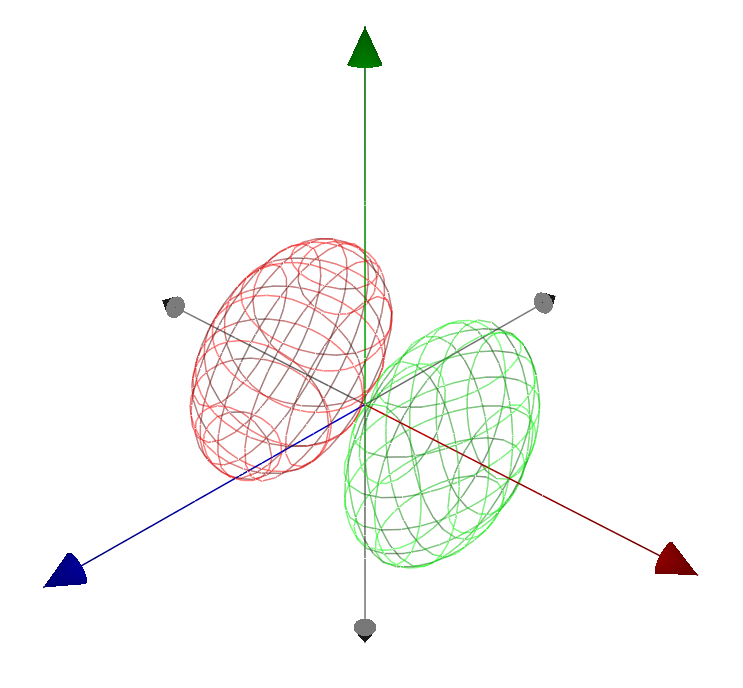
\includegraphics[scale=0.5]{RotatedSpheroid}
\caption{The rotation of a spheroid about the axis $(e_1+e_2+e_3)/\sqrt{3}$ by $\pi$ radians.}
\label{fig_rot_spheroid}
\end{figure}

To see that $V$ leaves $A$ invariant, notice that
\begin{equation}
VA\tilde{V} = Re_0\tilde{R}\wedge\overline{Re_0\tilde{R}}.
\end{equation}
We need only show now that $R$ leaves $e_0$ invariant.  To that end, we see that
\begin{align}
Re_0\tilde{R} &= \cos^2\frac{\theta}{2}e_0 + \cos\frac{\theta}{2}\sin\frac{\theta}{2}(e_0 aI - aIe_0) - \sin^2\frac{\theta}{2}aIe_0aI \\
 &= \cos^2\frac{\theta}{2}e_0 - \sin^2\frac{\theta}{2}(aI)^2 e_0 \\
 &= \left(\cos^2\frac{\theta}{2}+\sin^2\frac{\theta}{2}\right)e_0 = e_0,
\end{align}
since $|a|=1$.  Seeing that $V$ leaves $\Omega$ invariant is a bit trickier.  We first
observe that
\begin{equation}\label{equ_versor_acting_on_omega}
V\Omega\tilde{V} = \sum_{i=1}^n Re_i\tilde{R}\wedge\overline{R e_i\tilde{R}}.
\end{equation}
It is important to realize at this point that for all integers $i\in[1,n]$, that $e_i\neq Re_i\tilde{R}$,
yet $V$ really does leave $\Omega$ invariant.  To see why, we will rewrite $e_i$
in equation \eqref{equ_versor_acting_on_omega} as
\begin{equation}
e_i = \sum_{j=1}^n (e_i\cdot e_j)e_j.
\end{equation}
Now realize that
\begin{equation}
Re_i\tilde{R} = \sum_{j=1}^n (Re_i\tilde{R}\cdot e_j)e_j.
\end{equation}
It then follows that for any integer $i\in[1,n]$, we have
\begin{equation}
-e_i\wedge\overline{e_i}\cdot V\Omega\tilde{V} = \sum_{j=1}^n (Re_i\tilde{R}\cdot e_j)^2 = (Re_i\tilde{R})^2 = 1,
\end{equation}
showing that the coefficient of $e_i\wedge\overline{e_i}$ in $V\Omega\tilde{V}$ is 1.  Realize that
the application of a rotor leaves the magnitude of a vector unchanged.  To finish the proof, we
observe that for all integers $i\neq j$ in $[1,n]$, we have
\begin{equation}
-e_i\wedge\overline{e_j}\cdot V\Omega\tilde{V} =
\sum_{k=1}^n (Re_i\tilde{R}\cdot e_k)(Re_j\tilde{R}\cdot e_k)
= (Re_i\tilde{R})\cdot(Re_j\tilde{R}) = 0,
\end{equation}
showing that the coefficient of $e_i\wedge\overline e_j$ in $V\Omega\tilde{V}$ is 0.  Realize that
the action of a rotor taken with two orthogonal vectors does not change their orthogonal relationship.
It now follows that $V\Omega\tilde{V}=\Omega$.

If there is a versor that translates quadrics in our model, it is not at all obvious.
Rotations and translations in the conformal model can be developed together in
a very nice uniform way by first developing the ability to reflect any conformal
geometry about an arbitrary plane, which is really only about as hard as showing
that any conformal point can be reflected about such a plane.
It is easy to see that planes in our present model, as shown
in table \eqref{equ_canonical_forms_table}, are also versors.  Unlike the conformal
model, unfortunately, applying such versors to quadrics in our model does not
produce a reflection about the plane.  This doesn't mean, however, that we can't
find some way to translate quadrics in our model.

Given a direction vector $t\in\V$ and a quadric $E\in\G$, it is not at all hard
to show that the quadric $E'$, given by
\begin{equation}\label{equ_translate_quadric}
E' = E + (t\cdot E)\wedge e_0 + (\overline{t}\cdot E)\wedge\overline{e_0}
- (t\wedge\overline{t}\cdot E)\Alpha,
\end{equation}
represents the quadric $E$ translated by the direction vector $t$.  To see this,
simply expand the equation
\begin{equation}
0 = (p-t)\wedge\overline{(p-t)}\cdot E
\end{equation}
and then factor out $p\wedge\overline{p}$.
(It helps to realize that $\overline{t}\cdot E\in\V$ and $t\cdot E\in\overline{\V}$.)
Then, recalling
that $\Alpha=e_0\wedge\overline{e_0}$, the form $E'$ in equation \eqref{equ_translate_quadric}
begins to resemble what might be the result of a transformation of $E$ by some versor.
Exactly what versor this might be, however, if it even exists, remains to be seen.
If we could find a translation versor, we could combine such versors with
those of the form \eqref{equ_rotation_versor} to get the rigid body motions.
It may not be possible to do this, in which case we must conclude that
a better model for quadric surfaces exists.

\section{Flat Quadrics}

In the conformal model there is a distinction made between flat and round
geometries.  Interestingly, it can be seen that flats of the conformal model
are really just rounds taken to an infinite extreme.  For example, a plane
is simply a sphere centered at infinity with infinite radius.  Such geometries
of the conformal model have the property that $\infty$ is in the vector
sub-space of the blade representing the geometry.  We give here a
condition that we might use in the quadric model to test a given quadric
for its flatness.

For any given quadric $E\in\G$, let $f:\V\to\R$ be the function
\begin{equation}
f(x) = x\wedge\overline{x}\cdot E.
\end{equation}
Then, if for all pairs of homogenized affine points $a,b\in\V$
on $E$ we have
\begin{equation}
0=f(a-b),
\end{equation}
then $B$ is a flat quadric.  We really
should be mathematically precise here about what we mean when
we say that a given quadric is flat.  The reasoning behind this
condition, however, may suffice as adequate meaning.

Let $x\in\V$ be the direction vector $a-b$, and see that
\begin{equation}
0=f(a) = f(b+x) = f(b) + \nabla_x f(b) + f(a-b) = \nabla_x f(b),
\end{equation}
where $\nabla_x f(b)$ is the directional derivative of $f$ at $b$.
It follows that for any $b$ on $E$, the directional derivative of $f$ at $b$ in every
direction from $b$ to any other point $a$ on $E$ is zero.  Then, seeing that
$\nabla_x f(b)=x\cdot\nabla f(b)$, and that $\nabla f(b)$, (the gradient of
$f$ at $b$), is a direction vector orthogonal to the surface of the quadric at $b$,
it is clear that all other points $a$ on $E$ must be in the tangent space
of $E$ at $b$.  It follows that $E$ is flat in any neighborhood of a point
upon its surface.

Notice that under this criterion, lines, as they are considered flat in the conformal
model, are also considered flat under our present model.  To see this, notice that $f(w)=0$ when
$E$ is the line in table \eqref{equ_canonical_forms_table} and $w$ is any non-zero direction
vector parallel to the unit-length direction vector $v$.  Notice that cylinders are similarly
flat in such directions $w$, but clearly not in any other direction.

\section{Concluding Remarks}

While it has been shown that elements of $\G$ do indeed, under a given
definition, represent quadric surfaces, there really is nothing more or less
interesting about adding and subtracting these elements than adding and
subtracting vector equations whose solution sets represent the quadric surfaces.
There might not be any great advantage in using the elemental form over the
functional form.  There is some wonder, however, whether the model can
be helpful in studying what is referred to in \cite{Miller87}
and \cite{ZhiqiangXu05} as the pencil of two quadrics.
It would be particularly interesting if our model could provide a nice proof
that a ruled quadric must exist in the pencil of any two quadrics.
To begin to answer such a question, we would first need to know
how to classify ruled quadrics in $\G$.  These would appear to be the
quadrics $E\in\G$ that are flat in at least one direction on every point
of the surface.

That $\G$ was not something fancy like a Minkowski space or some other
type of non-Euclidean geometric algebra was perhaps our first clue from
the beginning that the potential for great things coming out of this model
was, let's say, less than likely.  On the other hand, it is very hard to see
all ends, and so perhaps there are deep results to be found or new insights
to be had using this method of studying quadric surfaces.  In any case,
geometric algebra has proven to be a fundamental, versatile and unifying
language that perhaps most naturally extends mathematics beyond the real number line.  Perhaps
there is a much better way to use geometric algebra to study quadric surfaces.
It is possible that as the model for projective geometry using geometric algebra may
be inferior to the conformal model, so the model of this paper may be inferior to
a conformal-like model for quadric surfaces.

\bibliographystyle{amsplain}
\bibliography{Parkin_QuadricSurfacesUsingGA}

\end{document}